\documentclass[]{article}

\usepackage{graphics}
\usepackage{geometry}
\usepackage{fontspec}
\usepackage{amsmath}
\usepackage{amssymb}
\usepackage{circuitikz}
\usepackage{minted2}

\setmainfont{NotoSans}
\geometry{margin=0.5in}
\graphicspath{{./images/}}
\DeclareGraphicsExtensions{.png}

\begin{document}

\author{Πλαστήρας Πέτρος}
\title{Εργαστήριο Λογικής Σχεδίασης - Εργασία 1}
\date{25 Νοεμβρίου 2024}
\maketitle
\section{Μέρος Β.2}

Παρακάτω σας δίνεται ο κώδικας VHDL για την περιγραφή της
οντότητας (entity) majority. Υλοποιήστε ένα κύκλωμα το οποίο θα δέχεται τρεις
εισόδους a, b, c και θα παράγει μια έξοδο y η οποία έχει την τιμή 1 όταν τουλάχιστον
δυο από τις εισόδους έχουν την τιμή 1.
\inputminted{vhdl}{majority.vhdl}

Προκειμένου να υλοποιήσουμε το κύκλωμα με τις παραπάνω προδιαγραφές πρέπει πρώτα να
σχεδιάσουμε τον πίνακα αληθείας της συνάρτησης που περιγράφεται και στην συνέχεια
χρησιμοποιώντας τον να δημιουργήσουμε και να απλοποιήσουμε τις εξισώσεις Boole που προκύπτουν.
\begin{center}
	\begin{tabular}{ | c | c | c | c | c | }
		\hline \rule{0pt}{11pt} $A$ & $B$ & $C$ & $Y$ & $m_i$                         \\
		\hline \rule{0pt}{11pt} 0   & 0   & 0   & 0   & $\bar{A} * \bar{B} * \bar{C}$ \\
		\rule{0pt}{11pt} 0          & 0   & 1   & 0   & $\bar{A} * \bar{B} * C$       \\
		\rule{0pt}{11pt} 0          & 1   & 0   & 0   & $\bar{A} * B * \bar{C}$       \\
		\rule{0pt}{11pt} 0          & 1   & 1   & 1   & $\bar{A} * B * C$             \\
		\rule{0pt}{11pt} 1          & 0   & 0   & 0   & $A * \bar{B} * \bar{C}$       \\
		\rule{0pt}{11pt} 1          & 0   & 1   & 1   & $A * \bar{B} * C$             \\
		\rule{0pt}{11pt} 1          & 1   & 0   & 1   & $A * B * \bar{C}$             \\
		\rule{0pt}{11pt} 1          & 1   & 1   & 1   & $A * B * C$                   \\
		\hline
	\end{tabular}
\end{center}

Από το παραπάνω προκύπτει ως άθροισμα γινομένων η παρακάτω εξίσωση για το $Y$:
$$ Y = \bar{A} * B * C + A * \bar{B} * C + A * B * \bar{C} + A * B * C$$

Χρησιμοποιώντας τα θεωρήματα της άλγεβρας Boole, μπορούμε να απλοποιήσουμε το παραπάνω ως εξής:
\begin{align*}
	Y & = \bar{A} * B * C + A * \bar{B} * C + A * B * \bar{C} + A * B * C \\
	  & = \bar{A} * B * C + A * \bar{B} * C + A * B * (\bar{C} + C)       \\
	  & = \bar{A} * B * C + A * \bar{B} * C + A * B * 1                   \\
	  & = \bar{A} * B * C + A * \bar{B} * C + A * B                       \\
	  & = \bar{A} * B * C + A * \bar{B} * C + A * B + A * B               \\
	  & = (\bar{A} * B * C + A * B) + (A * \bar{B} * C + A * B)           \\
	  & = (\bar{A} * C + A) * B + A * (\bar{B} * C + B)                   \\
	  & = (C + A) * B + A * (C + B)                                       \\
	  & = B * C + A * B + A * C + A * B                                   \\
	  & = B * C + A * B + A * C                                           \\
\end{align*}

Στην παραπάνω υλοποίηση χρησιμοποιούνται 3 AND και 2 OR πύλες. Μπορούμε να μειώσουμε τον αριθμό των πυλών που χρησιμοποιούνται εφαρμόζοντας την επιμεριστική ιδιότητα σε δύο από τους 3 όρους:
\begin{align*}
	Y & = B * C + A * B + A * C \\
	  & = B * (A + C) + A * C   \\
\end{align*}

Τώρα χρησιμοποιούνται 2 πύλες AND και 2 πύλες OR.
Μπορούμε επίσης να μειώσουμε τον αριθμό από CMOS transistors που χρησιμοποιούνται, εφαρμόζοντας κανόνες De Morgan ώστε να αλλάξουμε όσες πύλες γίνεται σε NOR και NAND:

\begin{align*}
	Y & = B * (A + C) + A * C                                  \\
	  & = \overline{\overline{B * (A + C)} * \overline{A * C}} \\
\end{align*}

Η παραπάνω είναι η τελική υλοποίηση που θα χρησιμοποιήσουμε. Αποτελείται από 3 πύλες NAND και μια πύλη OR.
Συνολικά έχει:
\begin{center}
	\begin{tabular}{| c | c |}
		\hline Πύλη   & Αριθμός CMOS Transistors \\
		\hline NAND-2 & 4                        \\
		NAND-2        & 4                        \\
		NAND-2        & 4                        \\
		OR-2          & 4 + 2 = 6                \\
		\hline Σύνολο & 4 + 4 + 4 + 6 = 18       \\
		\hline
	\end{tabular}
\end{center}

Ακολουθεί η υλοποίηση της οντότητας majority σε VHDL:
\begin{minted}{vhdl}
-- file majority.vhd
\end{minted}
\inputminted{vhdl}{./assign_1/majority.vhdl}

Μπορούμε τώρα να κάνουμε RTL ανάλυση του παραπάνω κώδικα. Πατώντας 'Open Elaborated Design'
προκύπτει το παρακάτω διάγραμμα:

\begin{center}
	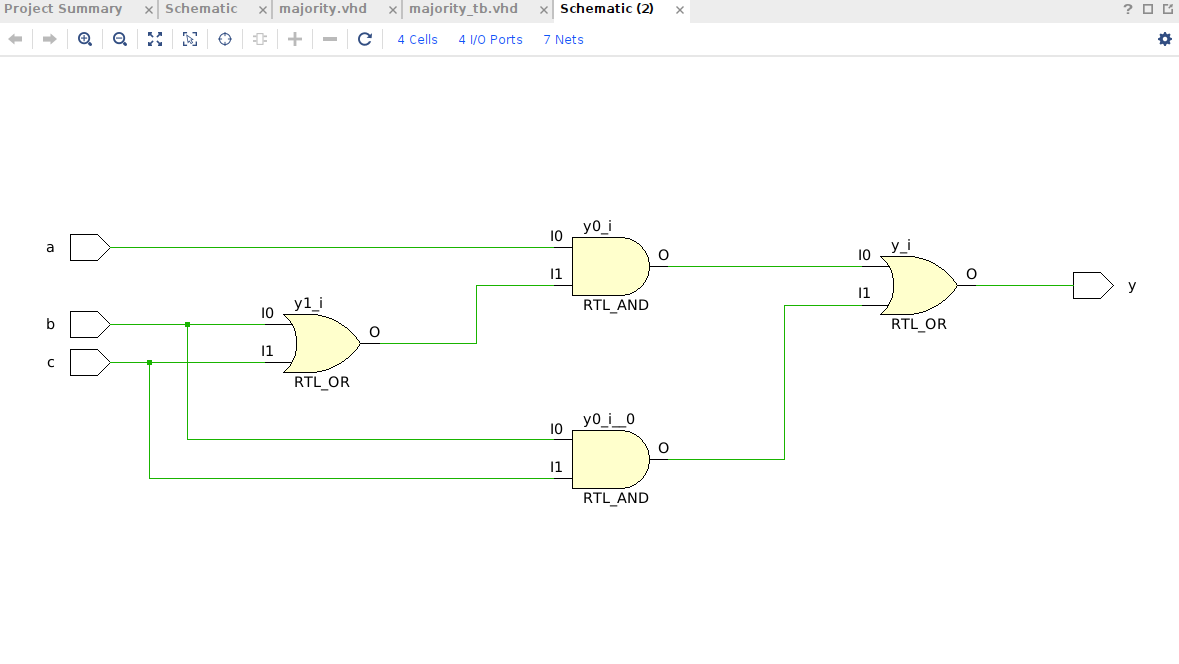
\includegraphics[width=\textwidth]{rtl_schem.png}
\end{center}

Όπως περιγράφηκε και παραπάνω, το κύκλωμα μας χρησιμοποιεί 3 πύλες NAND δύο εισόδων και 1 πύλη OR δύο εισόδων στην φάση της RTL ανάλυσης.

\newpage
Πλέον μπορούμε να κάνουμε σύνθεση και κάνοντάς την προκύπτει το παρακάτω διάγραμμα:

\begin{center}
	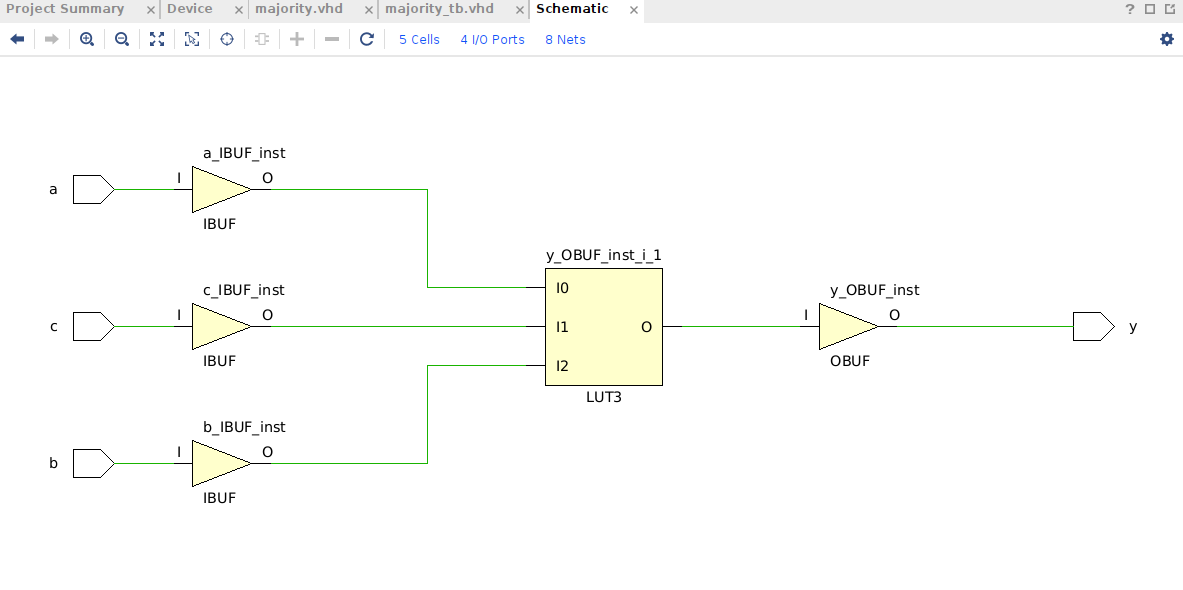
\includegraphics[width=\textwidth]{synthesis_schem.png}
\end{center}

% TODO: use a figure for the truth table so that we can reference it here
Στο παραπάνω φαίνεται η τελική υλοποίηση της οντότητας μας με χρήση look-up table(LUT). Χρησιμοποιούμε μόνο
1 look-up table τριών εισόδων, στο οποίο έχει αποθηκευτεί ο πίνακας αληθείας της συνάρτησης. Χρησιμοποι-
ούνται επίσης 3 buffers για την ενίσχυση των σημάτων a, b και c πριν την είσοδό τους στο LUT καθώς κι ένα επιπλέον buffer για την ενίσχυση της εξόδου y.

Για την προσομοίωση και τον έλεγχο της οντότητας majority υλοποιήθηκε και χρησιμοποιήθηκε η οντότητα majority\_tb με τον παρακάτω τρόπο:
\begin{minted}{vhdl}
-- file majority_tb.vhd
\end{minted}
\inputminted{vhdl}{./assign_1/majority_tb.vhdl}

% TODO: name of the first stage of simulation
Τρέχοντας το στάδιο του behavioral simulation προκύπτει η παρακάτω κυματομορφή:
\begin{center}
	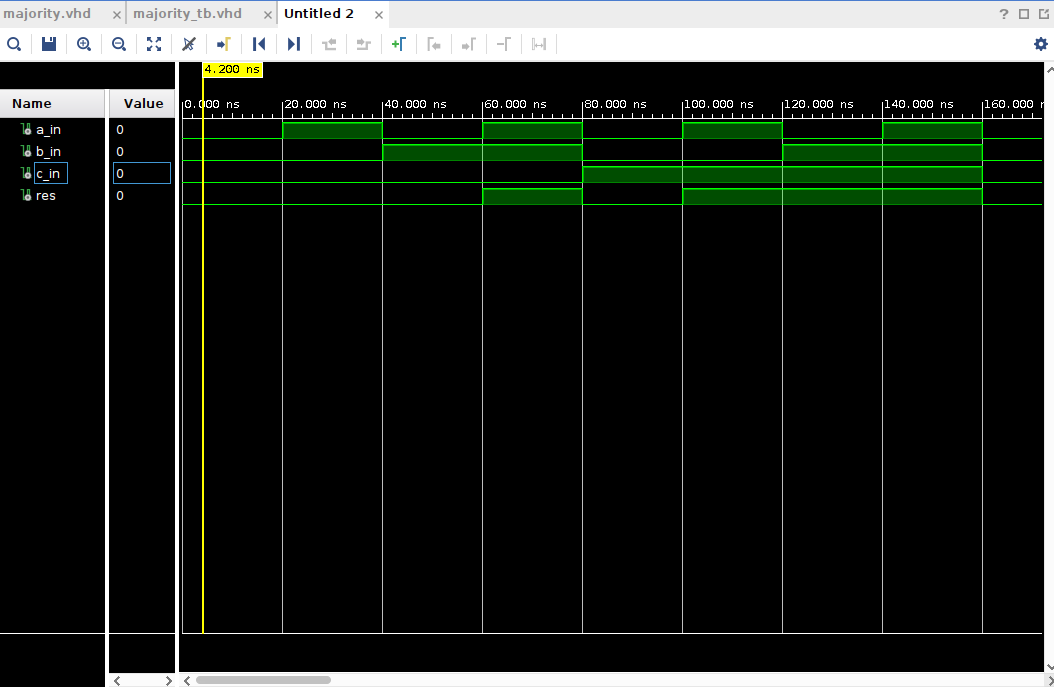
\includegraphics[width=\textwidth]{behavioral.png}
\end{center}

\newpage

Μιας που ήδη έχουμε εκτελέσει το στάδιο της σύνθεσης και του behavioral simulation μας δίνεται πλέον η επιλογή να κάνουμε Post Synthesis Timing Simulation.
Τρέχοντας το προκύπτει η παρακάτω κυματομορφή:
\begin{center}
	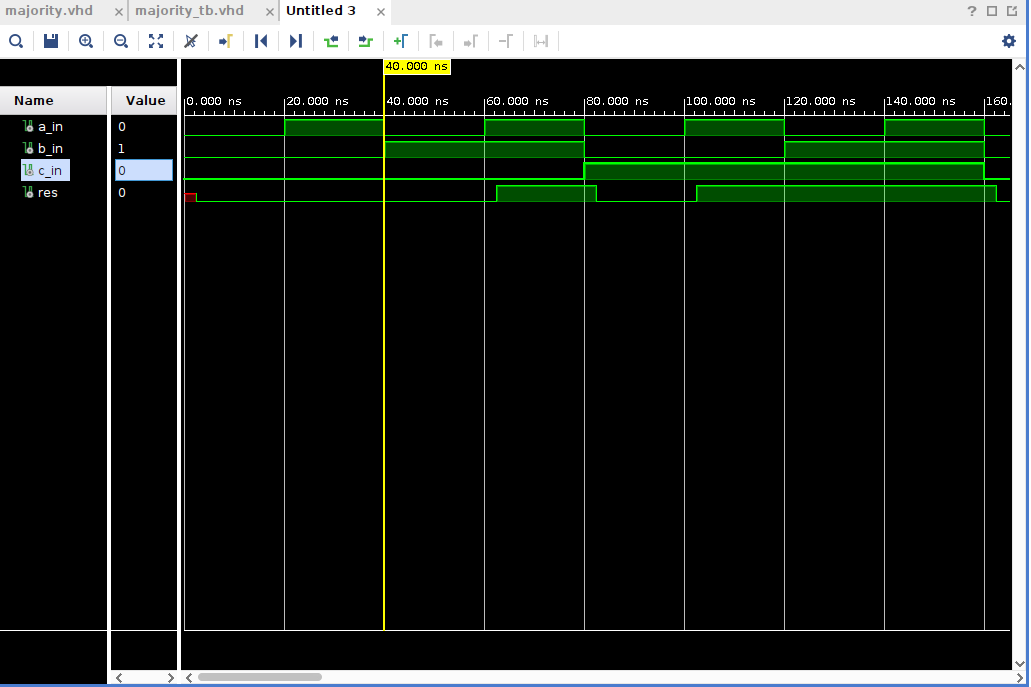
\includegraphics[width=\textwidth]{post_synthesis_timing.png}
\end{center}

Παρατηρείστε την διαφορά των δύο κυματομορφών. Ενώ στο behavioral simulation η μετάβαση από 0 σε 1 στο σήμα res γινόταν άμεσα εδώ
υπάρχει μια καθυστέρηση κατά την μεταβολή την τιμής του res, η οποία είναι της τάξης των $6ns$

\end{document}
